% !TEX program = xelatex

\documentclass[12pt,a4paper]{article}
\usepackage[UTF8]{ctex}
\usepackage{float}
\usepackage{amsmath}
\usepackage{amsfonts}
\usepackage{enumerate}
\usepackage{booktabs}
\usepackage{graphicx}
\usepackage{longtable}
\usepackage{subfigure}

\usepackage{url}
\usepackage{multirow}

% for plotting 
\usepackage{caption}
\usepackage{pgfplots}

% for pseudo code 
\usepackage{algorithm}
\usepackage[noend]{algpseudocode}

% for reference 
\usepackage{hyperref}
\usepackage{cleveref}

% for code 
\usepackage{listings}
\usepackage{xcolor}
\usepackage{fontspec}
\definecolor{darkgreen}{rgb}{0,0.6,0}
\newfontfamily\consolas{Consolas}

\usepackage{amssymb}
\usepackage{pifont}
\usepackage{xcolor}
\newcommand{\cmark}{\ding{51}}
\newcommand{\xmark}{\ding{55}}

\lstset {
    basicstyle=\footnotesize\consolas, % basic font setting
    breaklines=true, 
    frame=single,     % {single, shadowbox, bottomline}
    keywordstyle=\color{blue}, 
    commentstyle=\color{darkgreen},
    stringstyle=\color{red},
    showstringspaces=false,
    % backgroundcolor=\color{black!5}, % set backgroundcolor
    numbers=left, 
    numberstyle=\ttfamily,
}

% Microsoft Word A4 paper default layout 
\usepackage[a4paper, left=3.18cm, right=3.18cm, top=2.54cm, bottom=2.54cm]{geometry}

% \captionsetup[figure]{labelfont={bf}, name={Figure}}
% \captionsetup[table]{labelfont={bf}, name={Table}}

\crefname{equation}{方程}{方程}
\Crefname{equation}{方程}{方程}
\crefname{table}{表}{表}
\Crefname{table}{表}{表}
\crefname{figure}{图}{图}
\Crefname{figure}{图}{图}

\title{数学实验:第九次作业}
\author{计算机系 \quad 计73 \quad 2017011620 \quad 李家昊}
\date{\today}

% 实验报告格式的基本要求

% 系别、班级、学号、姓名

% 1 实验目的
% 2 题目
%   2.1 计算题:题号,算法设计(包括计算公式),程序,计算结果(计算机输出),结果分析,结论。
%   2.2 应用题:题号,问题分析,模型假设,模型建立,算法设计(包括计算公式),程序,计算结果(计算机输出),结果的数学分析,结果的实际意义,结论。
% 3 收获与建议

% Calc
% \subsubsection{算法设计}
% \subsubsection{程序}
% \subsubsection{计算结果}
% \subsubsection{结果分析}
% \subsubsection{结论}

% App
% \subsubsection{问题分析}
% \subsubsection{模型假设}
% \subsubsection{模型建立}
% \subsubsection{算法设计}
% \subsubsection{程序}
% \subsubsection{计算结果}
% \subsubsection{结果的数学分析}
% \subsubsection{结果的实际意义}
% \subsubsection{结论}

\begin{document}

\maketitle

\section{实验目的}

\begin{itemize}
    \item 掌握数据的参数估计、假设检验的基本原理、算法,及用MATLAB实现的方法。
    \item 练习用这些方法解决实际问题。
\end{itemize}

\section{问题求解}

\subsection{Chap12-Ex5 货物抽检(应用题)}

\subsubsection{算法设计}

\paragraph{模型建立} 设目标中心为$x=0,y=0$,圆形区域半径为$a=100$,则圆形区域可表示为$\Omega: x^2 + y^2 = a^2$,炮弹的落点服从二维正态分布$N(\boldsymbol{\mu}, \boldsymbol{\Sigma})$,其中,
\begin{equation}
    \boldsymbol{\mu} = \left(\begin{matrix}
        0\\
        0
    \end{matrix}\right)
    , \quad 
    \boldsymbol{\Sigma}  = \left(\begin{matrix}
        \sigma_x^2 & r \sigma_x \sigma_y \\
        r \sigma_x \sigma_y & \sigma_y^2
    \end{matrix}\right)
\end{equation}

记$\boldsymbol{x} = (x,y)^T$,其维度$m=2$,则概率密度函数如下,图像如\Cref{fig:ex5_pdf}。
\begin{equation}
    f(\boldsymbol{x})=\left(\frac{1}{2 \pi}\right)^{\frac{m}{2}} \frac{1}{\sqrt{|\boldsymbol{\Sigma|}}} \exp \left[-\frac{1}{2}(\boldsymbol{x}-\boldsymbol{\mu})^{T} \boldsymbol{\Sigma}^{-1}(\boldsymbol{x}-\boldsymbol{\mu})\right]
\end{equation}

炮弹命中圆形区域内部的概率$p$为,
\begin{equation}\label{eq:ex5_model}
    p = \iint_\Omega f(x,y) dxdy
\end{equation}

\Cref{eq:ex5_model}即为本题的模型。

\begin{figure}[H]
    \centering
    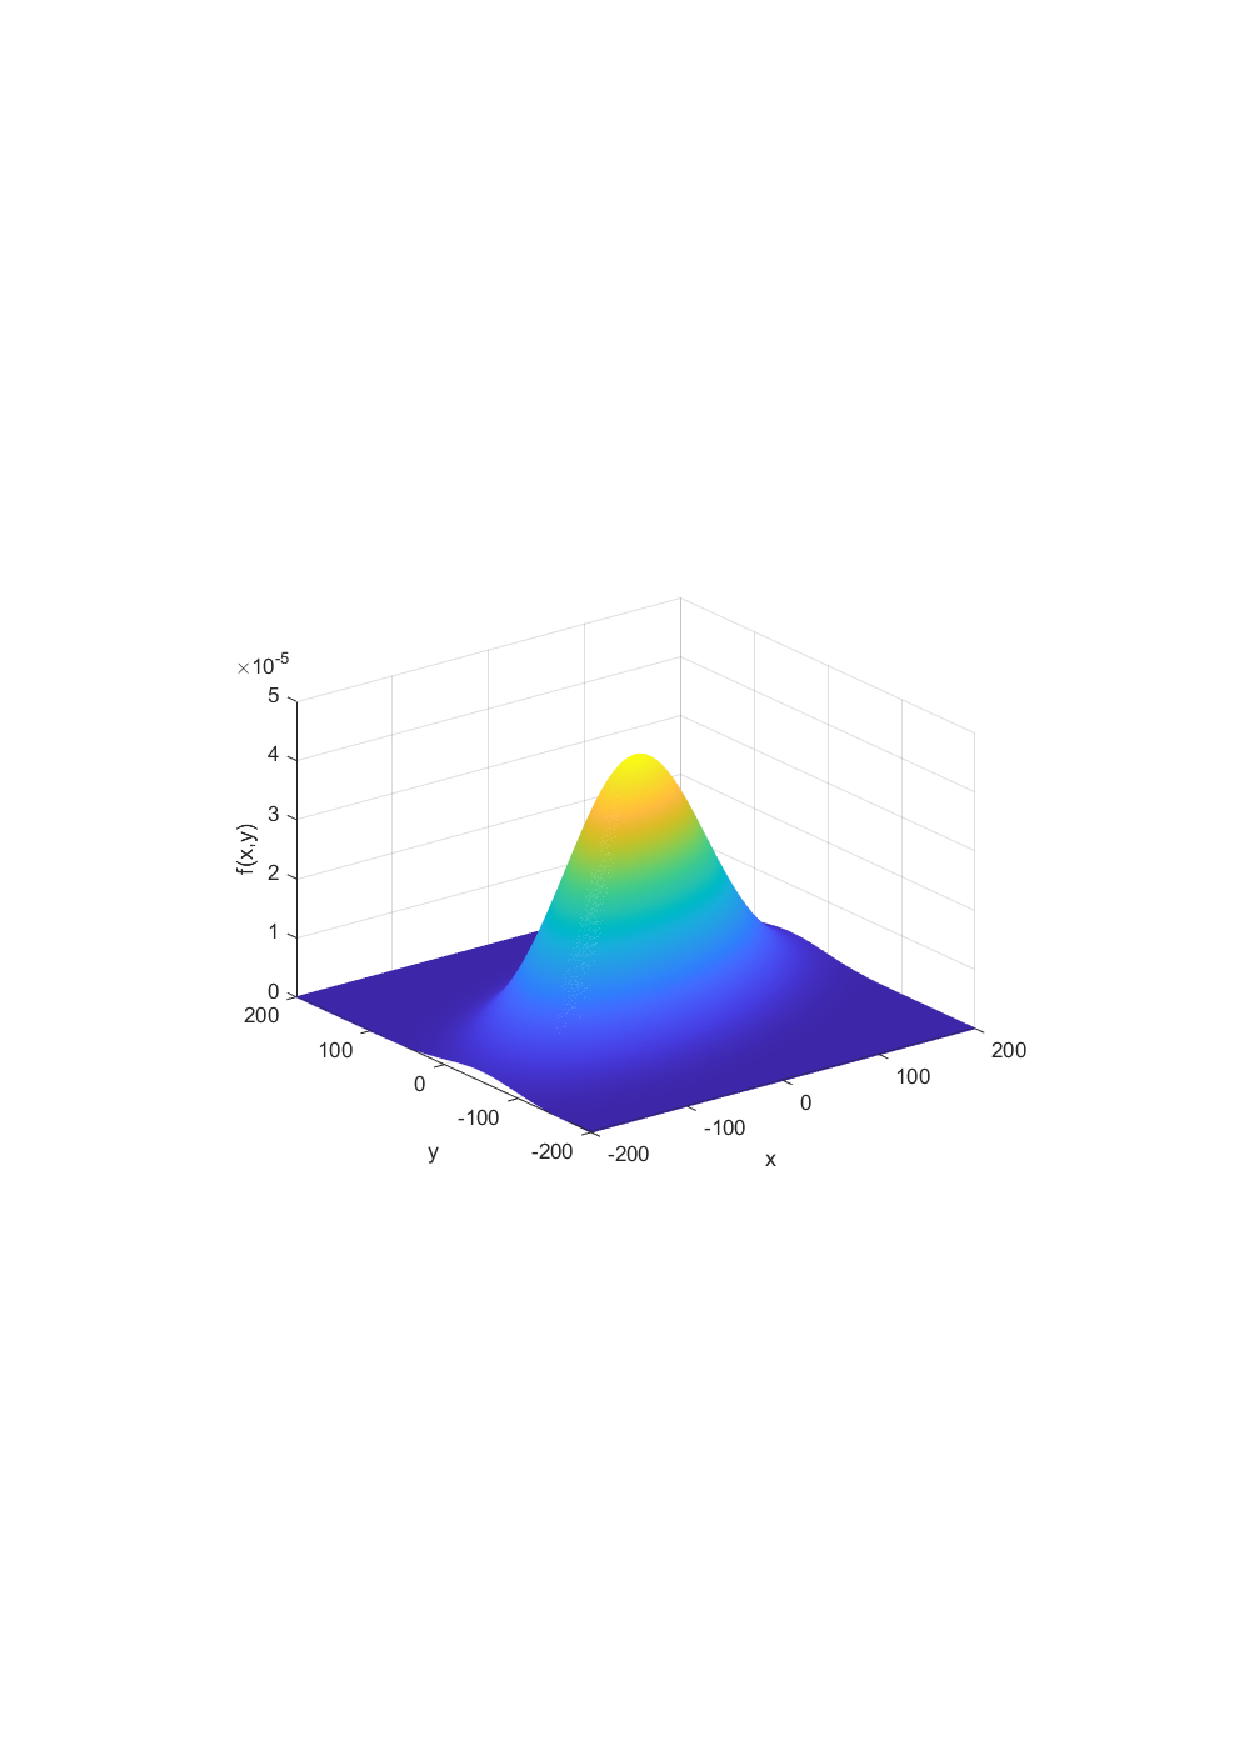
\includegraphics[width=0.8\textwidth,trim={3.09cm 9.295cm 3.09cm 9.295cm},clip]{fig/ex5_pdf.pdf}
    \caption{概率密度函数$f(x,y)$的图像}
    \label{fig:ex5_pdf}
\end{figure}

\paragraph{算法实现} 考虑到\Cref{eq:ex5_model}的二重积分无解析解,可以采用两种方法求解。

一种方法是采用蒙特卡洛方法求解,取$n$个独立均匀分布在区域$[-a,a]\times [-a,a]$的随机点$\{(x_i,y_i)\}_{i=1}^n$,记$I$为示性函数,则可近似计算得出,
\begin{equation}
    p = \frac{4a^2}{n} \sum_{i=1}^n f(x_i, y_i) I_{(x_i, y_i) \in \Omega}
\end{equation}

另一种方法是采用数值积分方法求解,即,
\begin{equation}
    p = \int_{-a}^a \int_{-a}^a f(x,y) I_{(x, y) \in \Omega} dxdy
\end{equation}

在MATLAB的实现中,可采用\texttt{mvnpdf}命令计算二维正态分布的概率密度函数$f$,采用\texttt{unifrnd}命令生成独立均匀分布的随机数,采用\texttt{integral2}命令计算二维数值积分。

\subsubsection{程序}

请参见附录\ref{sec:ex5_code}。

\subsubsection{计算结果}

\paragraph{蒙特卡洛方法} 分别选取$n=10^4,10^5,10^6,10^7$,在每个$n$值下计算5次,得到结果如\Cref{tab:ex5_results}。取$n=10^7$时5次计算的均值作为最终结果,得到$p=0.6980$。

\begin{table}[H]
    \centering
    \caption{不同$n$取值下计算5次得到的概率$p$值}
    \label{tab:ex5_results}
    \begin{tabular}{c|ccccc|cc}
        \toprule
        $n$ & 1 & 2 & 3 & 4 & 5 & Mean & Variance\tabularnewline
        \midrule
        $10^4$ & 0.7032 & 0.7030 & 0.6991 & 0.6903 & 0.7019 & 0.6995 & $2.9125\times 10^{-5}$\tabularnewline
        $10^5$ & 0.6977 & 0.6962 & 0.6970 & 0.6978 & 0.7014 & 0.6980 & $3.9820\times 10^{-6}$\tabularnewline
        $10^6$ & 0.6973 & 0.6985 & 0.6978 & 0.6979 & 0.6986 & 0.6980 & $2.8700\times 10^{-7}$\tabularnewline
        $10^7$ & 0.6980 & 0.6981 & 0.6977 & 0.6979 & 0.6984 & 0.6980 & $6.7000\times 10^{-8}$\tabularnewline
        \bottomrule
    \end{tabular}
\end{table}

\paragraph{数值积分方法} 利用数值积分方法求出的值为$p=0.6980$。

\subsubsection{结果分析}

从\Cref{tab:ex5_results}可以看出,采用蒙特卡洛方法时,随着试验次数$n$的增大,计算结果的方差逐渐减小,逐步稳定在真值附近,当$n$达到$10^5$时,蒙特卡洛结果与数值积分结果已经非常接近,可作为真值的一个近似解。

\subsubsection{结论}

炮弹命中圆形区域的概率为69.80\%。


\subsection{Chap12-Ex6 身高体重(计算题)}

% 6. 学校随机抽取100名学生,测量他们的身高和体重,所得数据如表12.6。
% 1)	对这些数据给出直观的图形描述,检验分布的正态性;
% 2)	根据这些数据对全校学生的平均身高和体重做出估计,并给出估计的误差范围;
% 3)	学校10年前作过普查,学生的平均身高为167.5厘米,平均体重为60.2公斤,根据这次抽查的数据,对学生的平均身高和体重有无明显变化做出结论。

\subsubsection{算法设计}

\paragraph{第(1)问} 首先检验总体分布的正态性,题目给出了100名学生的身高和体重数据,样本量不小,可采用Jarque-Bera检验和Lilliefors检验,对应的MATLAB命令分别为\texttt{jbtest}和\texttt{lillietest};然后进行数据可视化,使用\texttt{histfit}命令画出频率分布直方图并拟合正态曲线。

\paragraph{第(2)问} 对于正态分布的参数估计,可使用\texttt{normfit}命令,根据给定的显著性水平,对总体均值$\mu$和方差$\sigma$进行点估计和区间估计。

\paragraph{第(3)问} 题目给出了10年前的总体均值$\mu_0$,采用单总体均值的假设检验方法,记原假设$H_0$和对立假设$H_1$为,
\begin{equation}
    H_0: \mu = \mu_0, \quad H_1: \mu \ne \mu_0
\end{equation}

由于总体方差未知,故采用$t$检验,对应的MATLAB命令为\texttt{ttest}。若原假设$H_0$被接受,则10年来学生身高体重无明显变化,反之,则发生了显著变化。

\subsubsection{程序}

请参见附录\ref{sec:ex6_code}。

\subsubsection{计算结果}

\paragraph{第(1)问} 在默认的显著性水平(0.05)下,Jarque-Bera检验和Lilliefors检验均表明,身高和体重两个总体均服从正态分布。作出频率分布直方图及拟合的正态曲线,如\Cref{fig:ex6_histfit},可以看出,身高体重的频率分布基本符合正态分布曲线。

\begin{figure}[H]
    \centering
    \subfigure[身高分布]{
        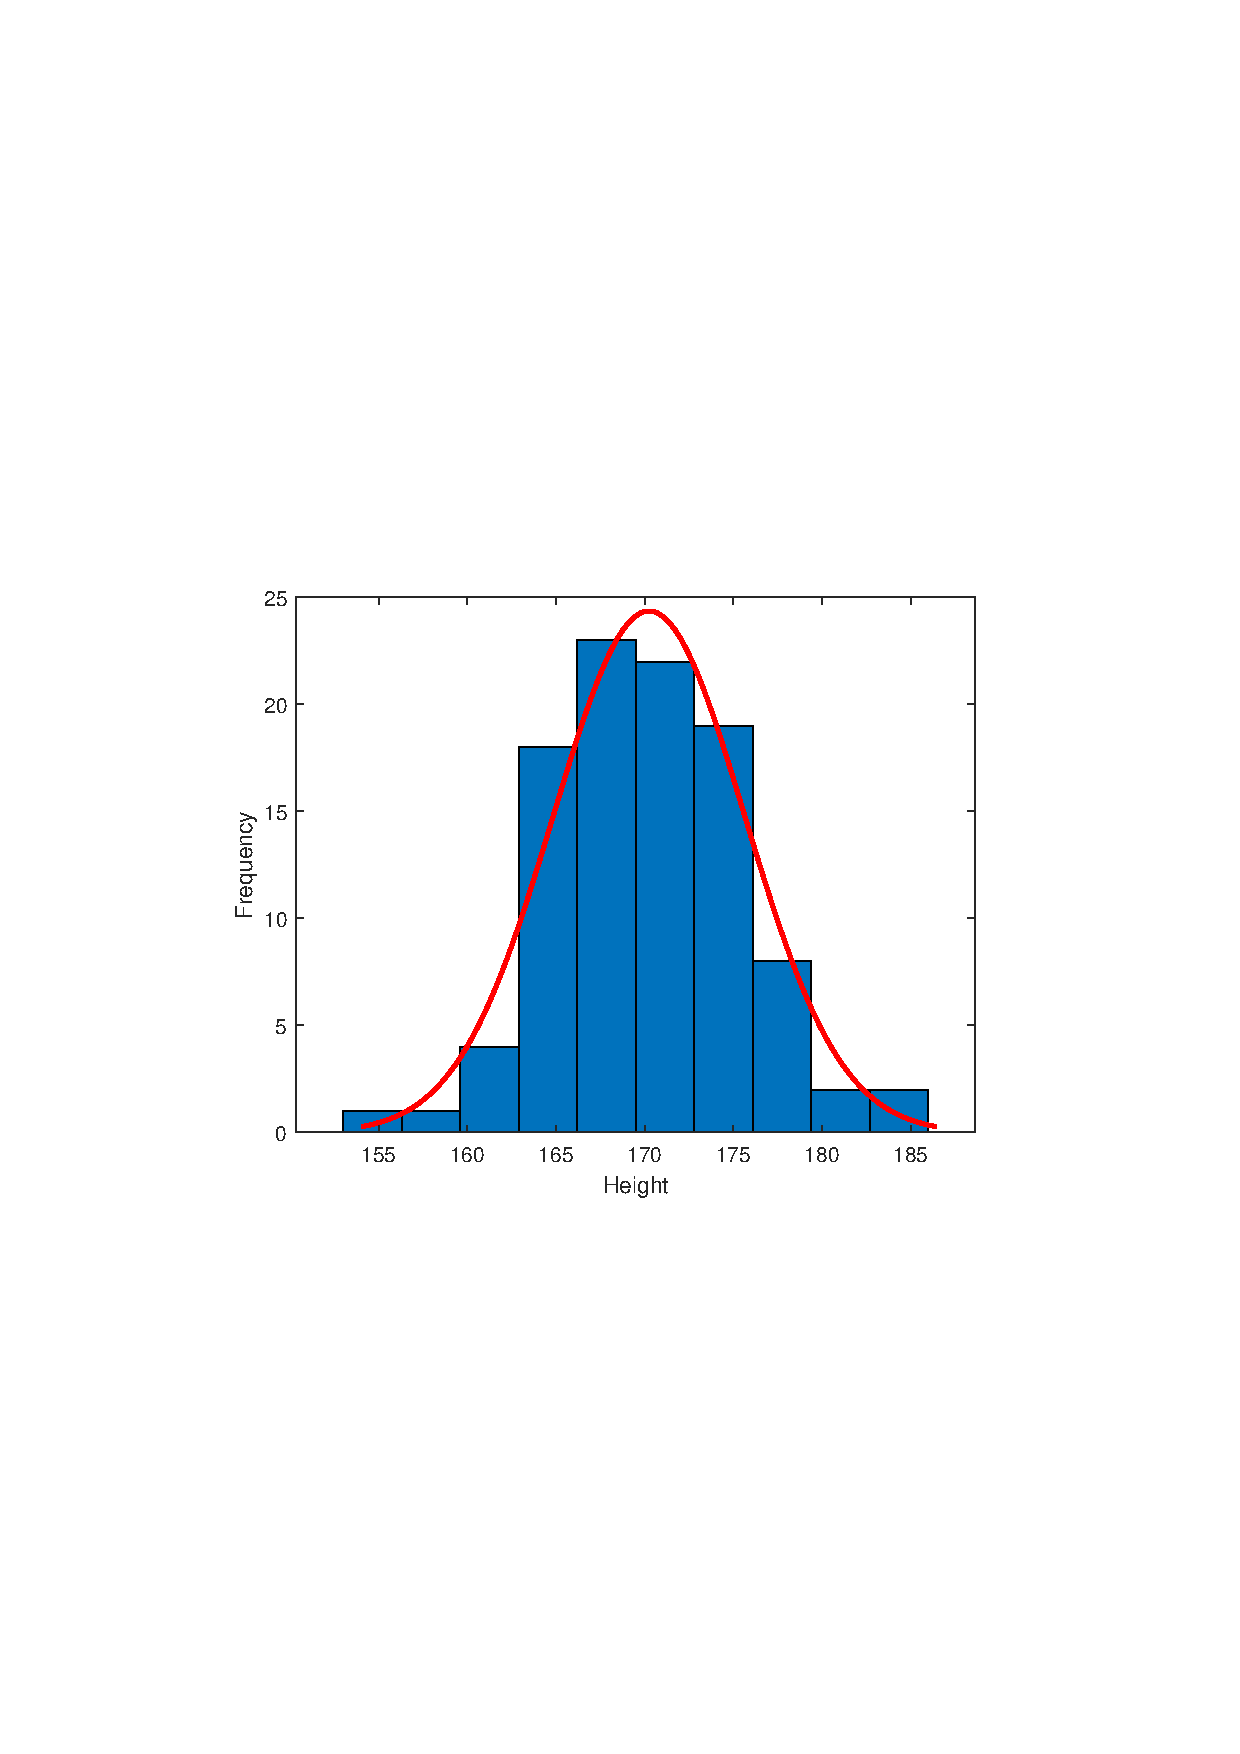
\includegraphics[width=0.47\textwidth,trim={3.09cm 9.295cm 3.09cm 9.295cm},clip]{fig/ex6_height_histfit.pdf}
    }
    \subfigure[体重分布]{
        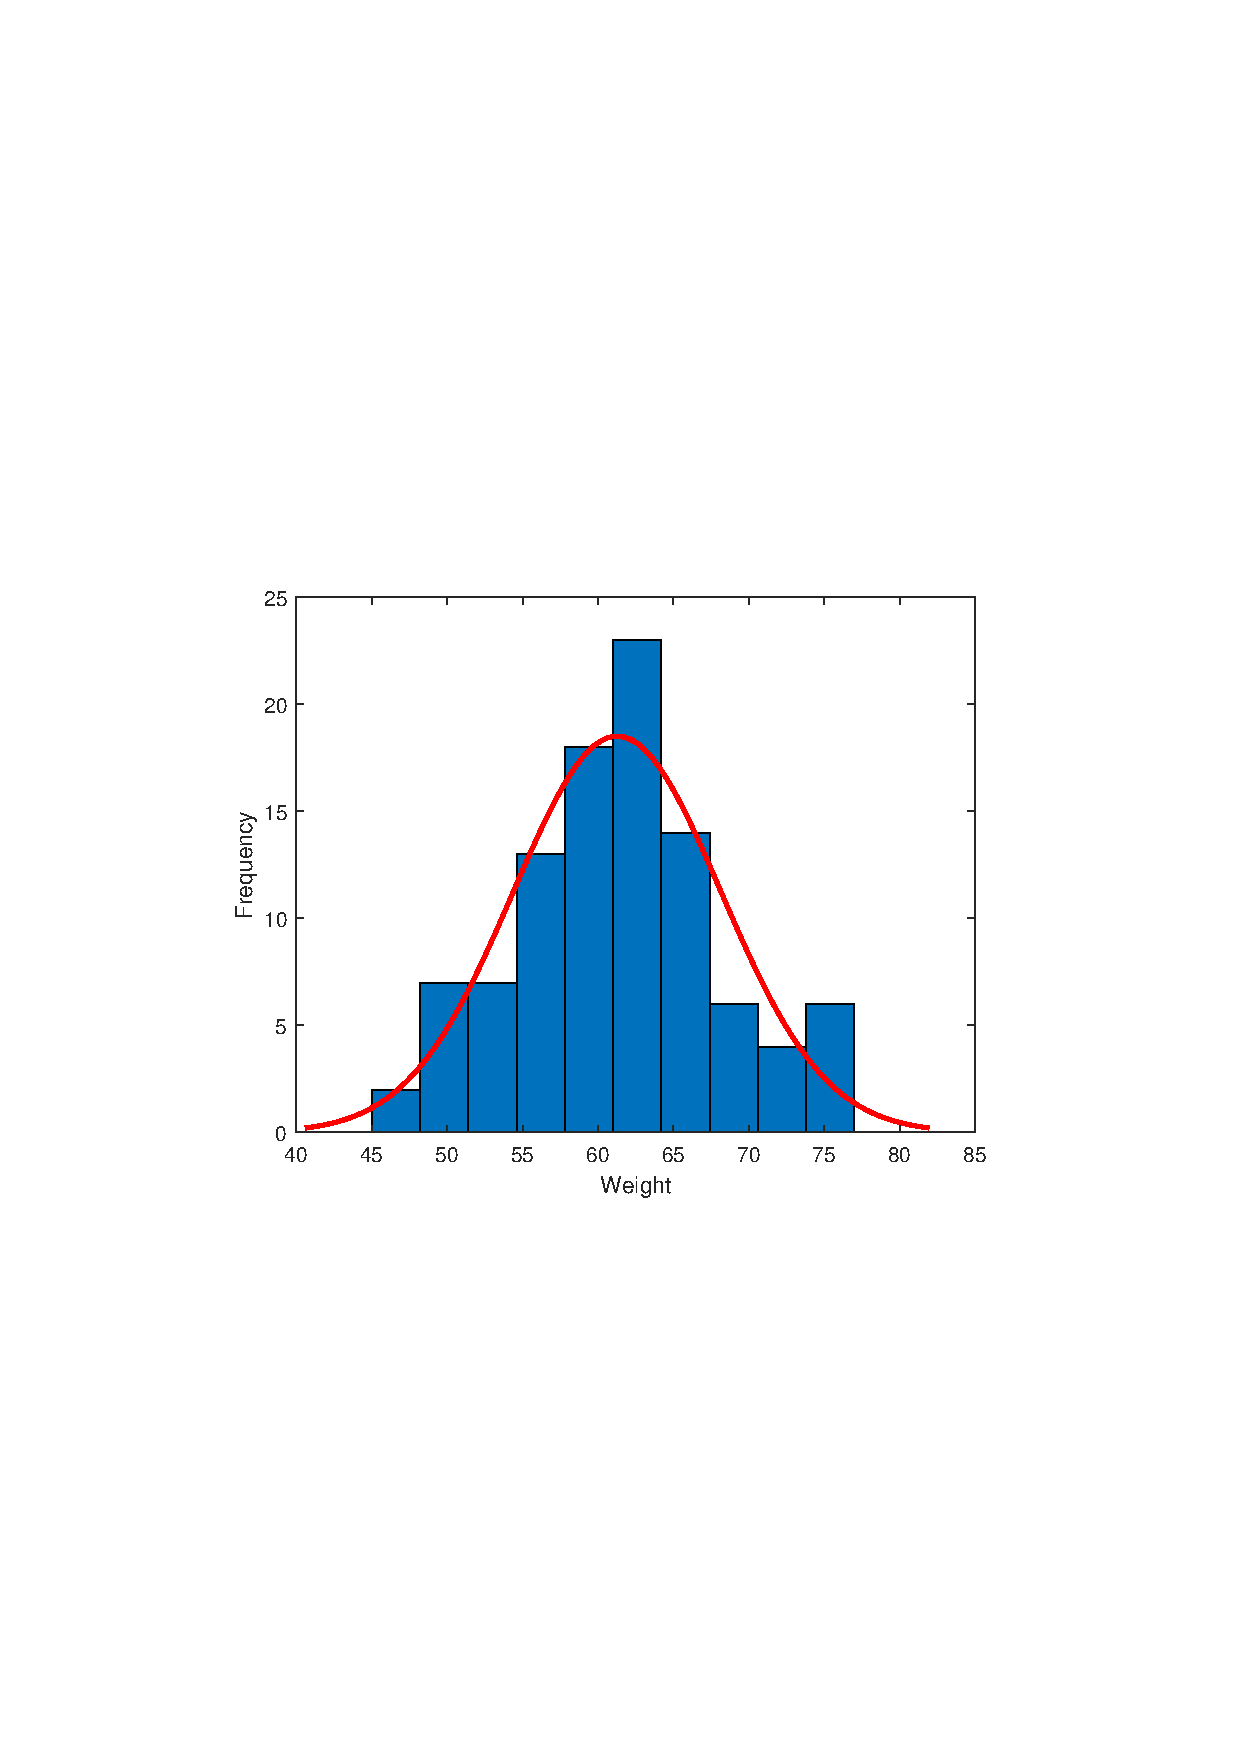
\includegraphics[width=0.47\textwidth,trim={3.09cm 9.295cm 3.09cm 9.295cm},clip]{fig/ex6_weight_histfit.pdf}
    }
    \caption{学生身高和体重的频率分布直方图及拟合的正态曲线}
    \label{fig:ex6_histfit}
\end{figure}

\paragraph{第(2)问} 在默认的显著性水平(0.05)下,身高和体重两个总体的参数估计如\Cref{tab:ex6_normfit},其中包括均值和方差的点估计和区间估计。在不同的显著性水平下,身高和体重的置信区间如\Cref{fig:ex6_height_alpha}和\Cref{fig:ex6_weight_alpha}。

\begin{table}[H]
    \centering
    \caption{身高和体重分布的参数估计}
    \label{tab:ex6_normfit}
    \begin{tabular}{c|ccccc}
        \toprule
        指标 & 均值点估计 & 标准差点估计 & 均值区间估计 &
        标准差区间估计\tabularnewline
        \midrule
        身高 (cm) & 170.25 & 5.40 & [169.18, 171.32] & [4.74,
        6.28]\tabularnewline
        体重 (kg) & 61.27 & 6.89 & [59.90, 62.64] & [6.05,
        8.01]\tabularnewline
        \bottomrule
    \end{tabular}
\end{table}

\begin{figure}[t]
    \centering
    \subfigure[均值置信区间]{
        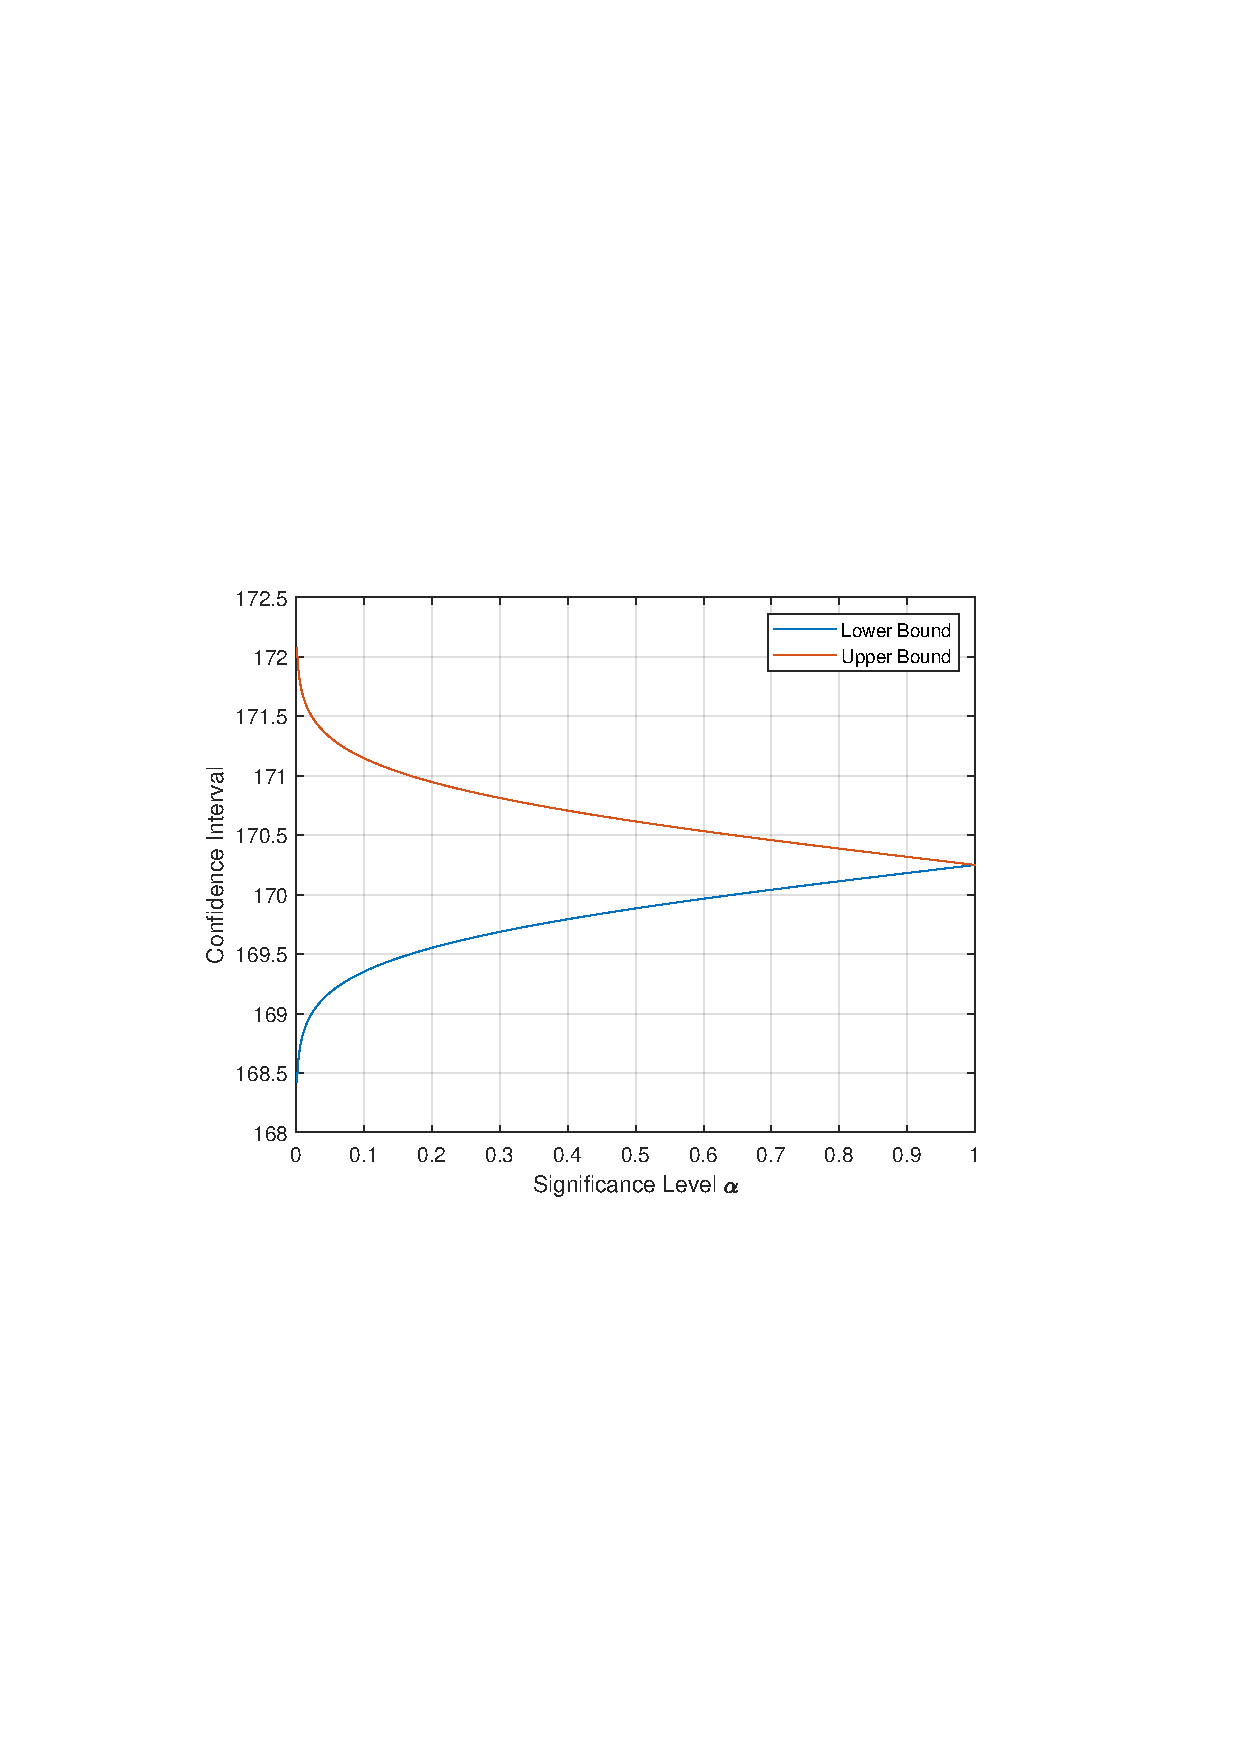
\includegraphics[width=0.47\textwidth,trim={3.09cm 9.295cm 3.09cm 9.295cm},clip]{fig/ex6_height_mu_alpha.pdf}
    }
    \subfigure[方差置信区间]{
        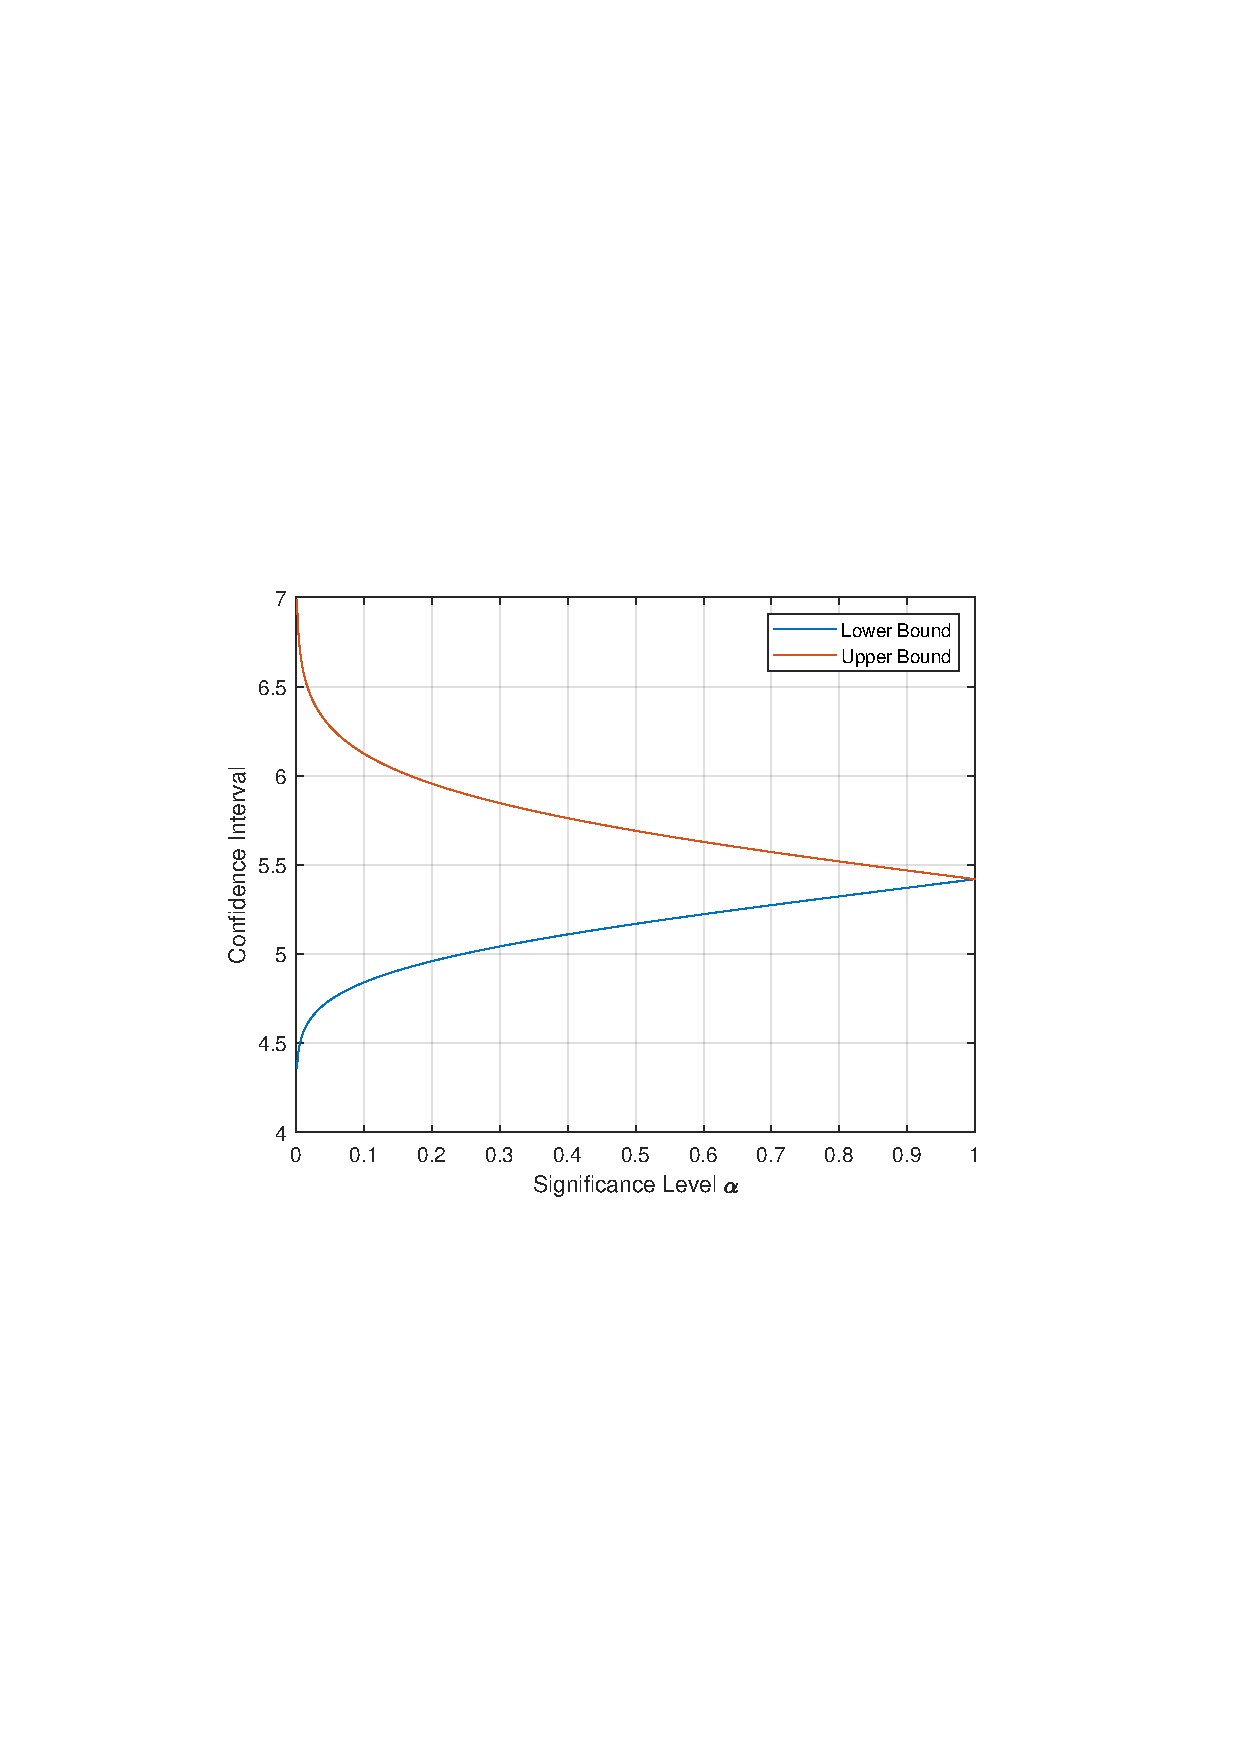
\includegraphics[width=0.47\textwidth,trim={3.09cm 9.295cm 3.09cm 9.295cm},clip]{fig/ex6_height_sigma_alpha.pdf}
    }
    \caption{不同的显著性水平下,身高的总体均值和方差的置信区间}
    \label{fig:ex6_height_alpha}
\end{figure}

\begin{figure}[t]
    \centering
    \subfigure[均值置信区间]{
        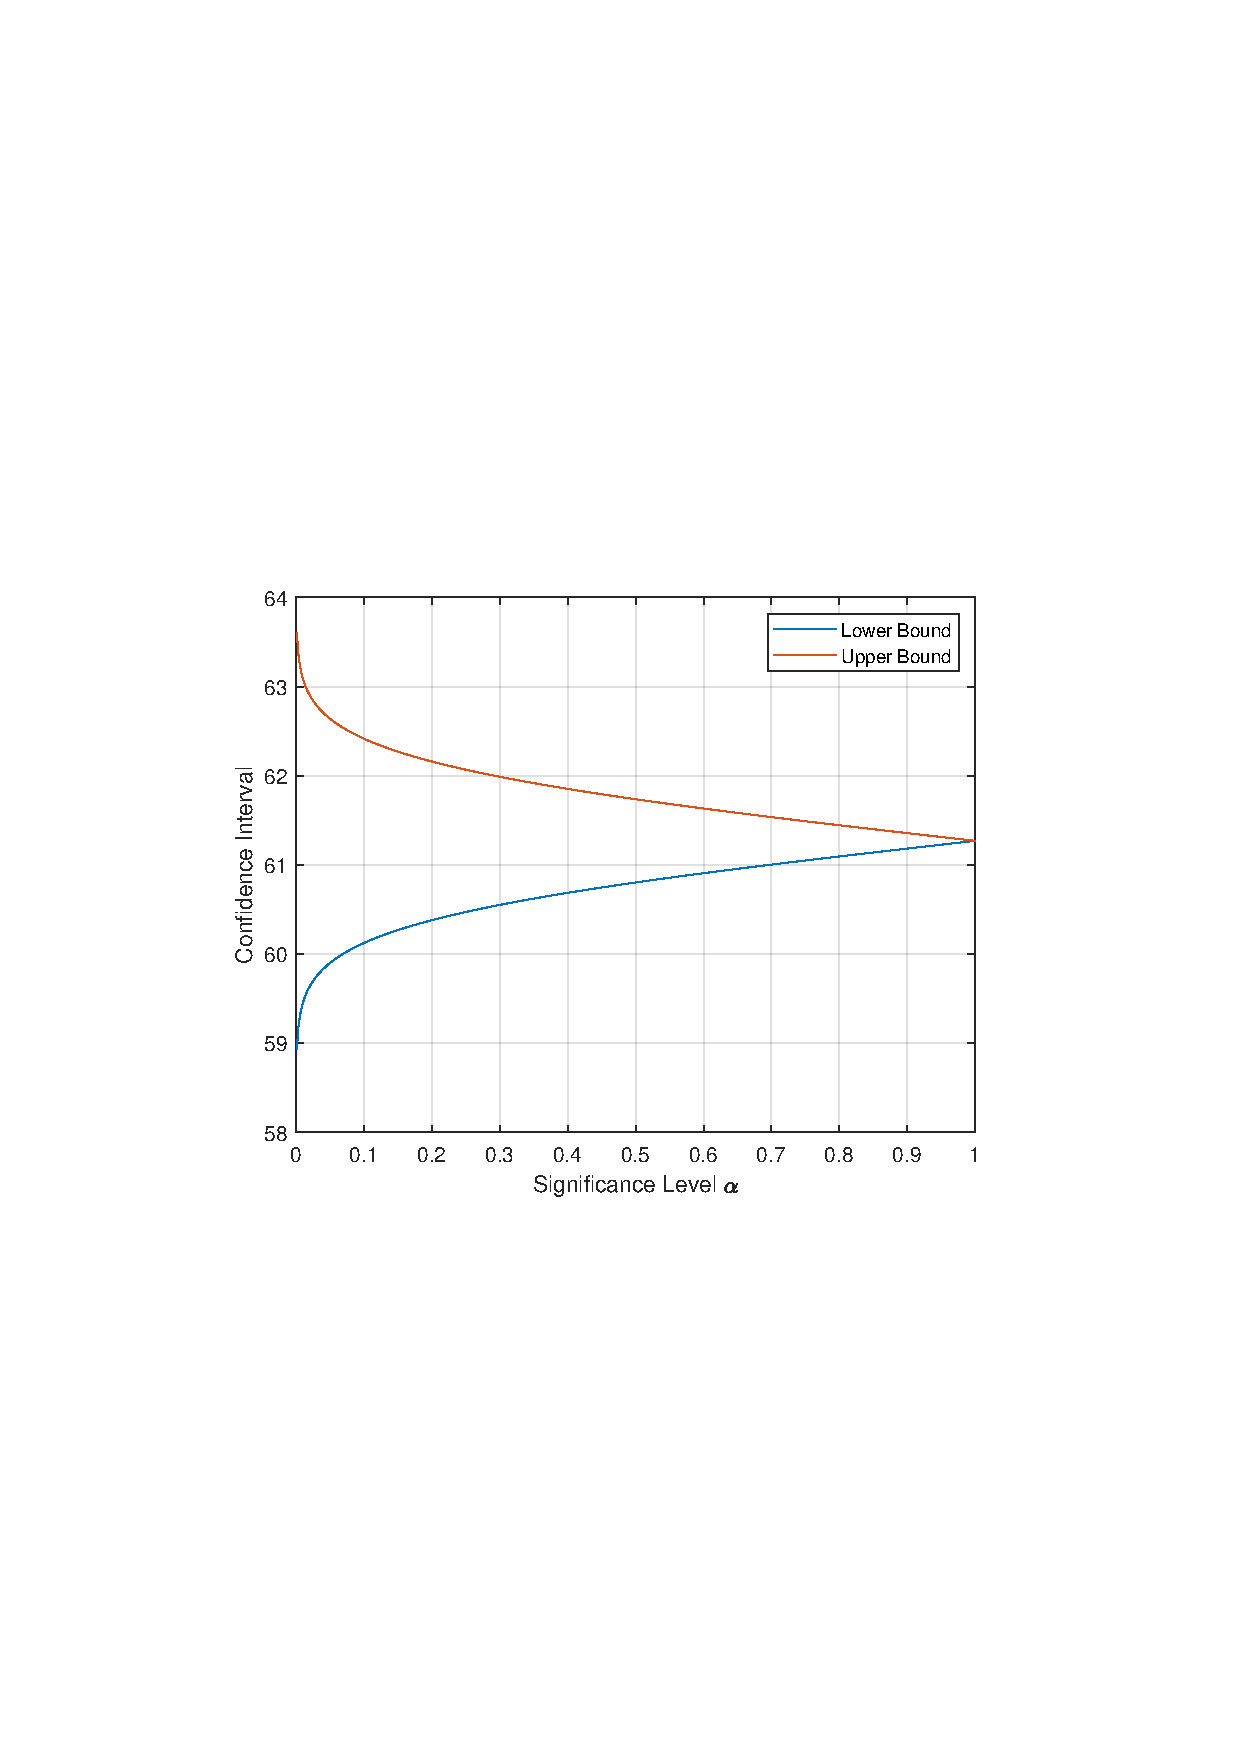
\includegraphics[width=0.47\textwidth,trim={3.09cm 9.295cm 3.09cm 9.295cm},clip]{fig/ex6_weight_mu_alpha.pdf}
    }
    \subfigure[方差置信区间]{
        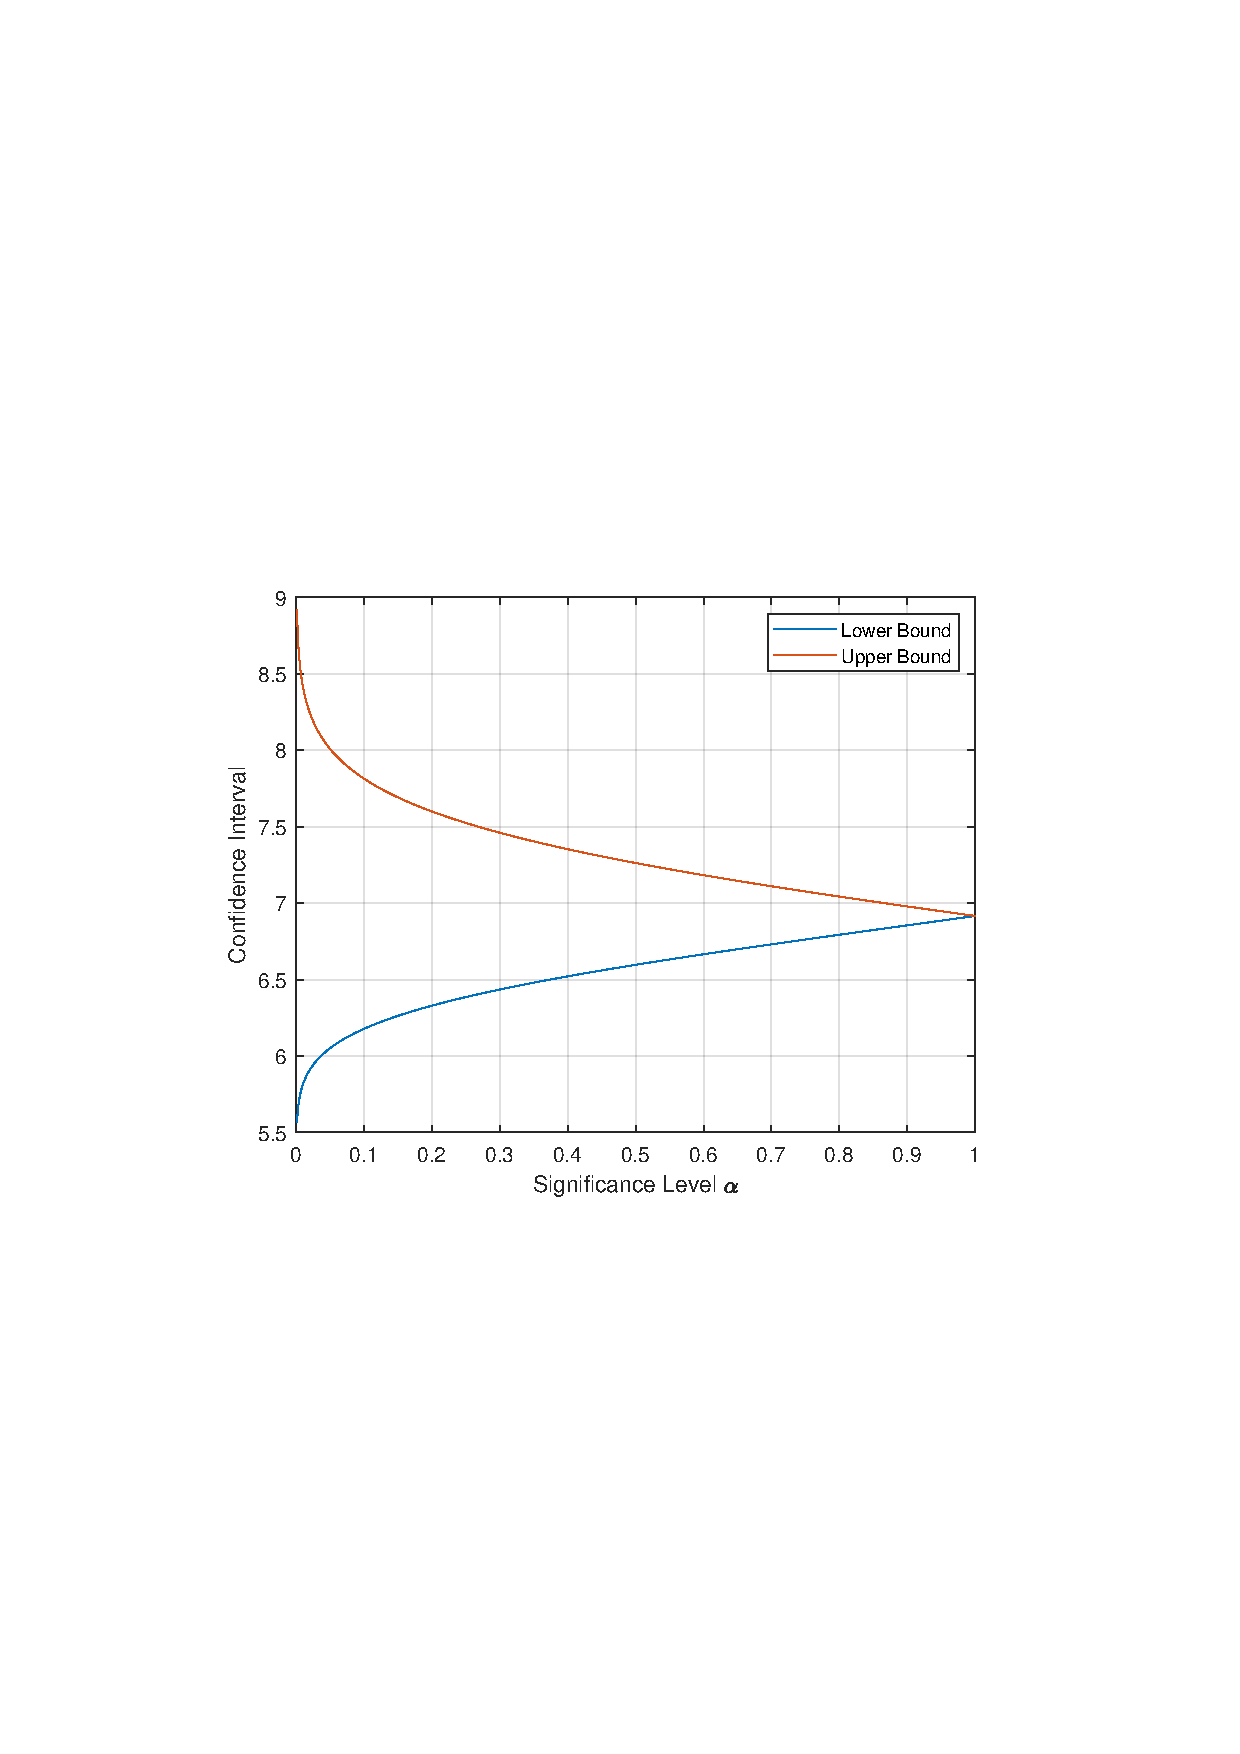
\includegraphics[width=0.47\textwidth,trim={3.09cm 9.295cm 3.09cm 9.295cm},clip]{fig/ex6_weight_sigma_alpha.pdf}
    }
    \caption{不同的显著性水平下,体重的总体均值和方差的置信区间}
    \label{fig:ex6_weight_alpha}
\end{figure}

\paragraph{第(3)问} 在默认的显著性水平(0.05)下,经过$t$检验,身高总体的原假设不成立,体重总体的原假设成立,由此可以断定,近10年来,学生的平均身高发生了明显变化,而平均体重无明显变化。

\subsubsection{结果分析}

从\Cref{fig:ex6_histfit}可以看出,在较大的样本量下,学生的身高和体重近似服从正态分布,这与概率论的中心极限定理相吻合。

从\Cref{fig:ex6_height_alpha}和\Cref{fig:ex6_weight_alpha}可以看出,当显著性水平趋于0时,置信区间长度趋于无穷;当显著性水平趋于1时,置信区间长度趋于0,收敛到点估计值;随着显著性水平的增加,即置信概率的降低,参数的置信区间随之缩小。计算结果与理论分析相符。

\subsubsection{结论}

在95\%的置信概率下,全校学生的身高和体重均服从正态分布,如\Cref{fig:ex6_histfit}。

全校学生的平均身高为170.25厘米,平均体重为61.27千克,在95\%的置信概率下,平均身高处于置信区间[169.18, 171.32]内,平均体重处于置信区间[59.90, 62.64]内。

在95\%的置信概率下,近10年来,学生的平均身高发生了明显变化,而平均体重无明显变化。


\subsection{Chap12-Ex7 胃溃疡病理(应用题)}

\subsubsection{算法设计}

\paragraph{模型建立} 记报童每天购入报纸数量为$n$,需求量为$r$,服从正态分布$N(\mu, \sigma^2)$,其概率密度函数为$f$,批发价为$a=A(1-n/K)$,每份报纸的零售价为$b$,退回价为$c$,则报童每天的利润$V$为,
\begin{equation}\label{eq:ex7_profit}
    V(n)=\sum_{r=0}^{n-1}[(b-a) r-(a-c)(n-r)] f(r)+\sum_{r=n}^{\infty}[(b-a) n] f(r)
\end{equation}

其图像如\Cref{fig:ex7_profit},可以看到,随着购入报纸数量$n$的增大,利润$V$首先在$n=2000$附近出现了一个极大值,然后降低到负值,然而,随着$n$的继续增大,$V$的值出现了急速的攀升,甚至超过了之前的极大值。这是因为随着$n$的增大,批发价格$a$逐渐降低,当$n>15000$时,批发价格竟然低于回收价格,当$n>50000$时,批发价格甚至变成了负数,在这些情况下,报童只要多购进报纸,再统一进行回收,就能赚到差价,显然是不符合实际情况的。为了保证批发价与回收价之间有一定的差价,这里对$n$的范围做如下规定,
\begin{equation}
    0 \le n \le 5000
\end{equation}

\begin{figure}[H]
    \centering
    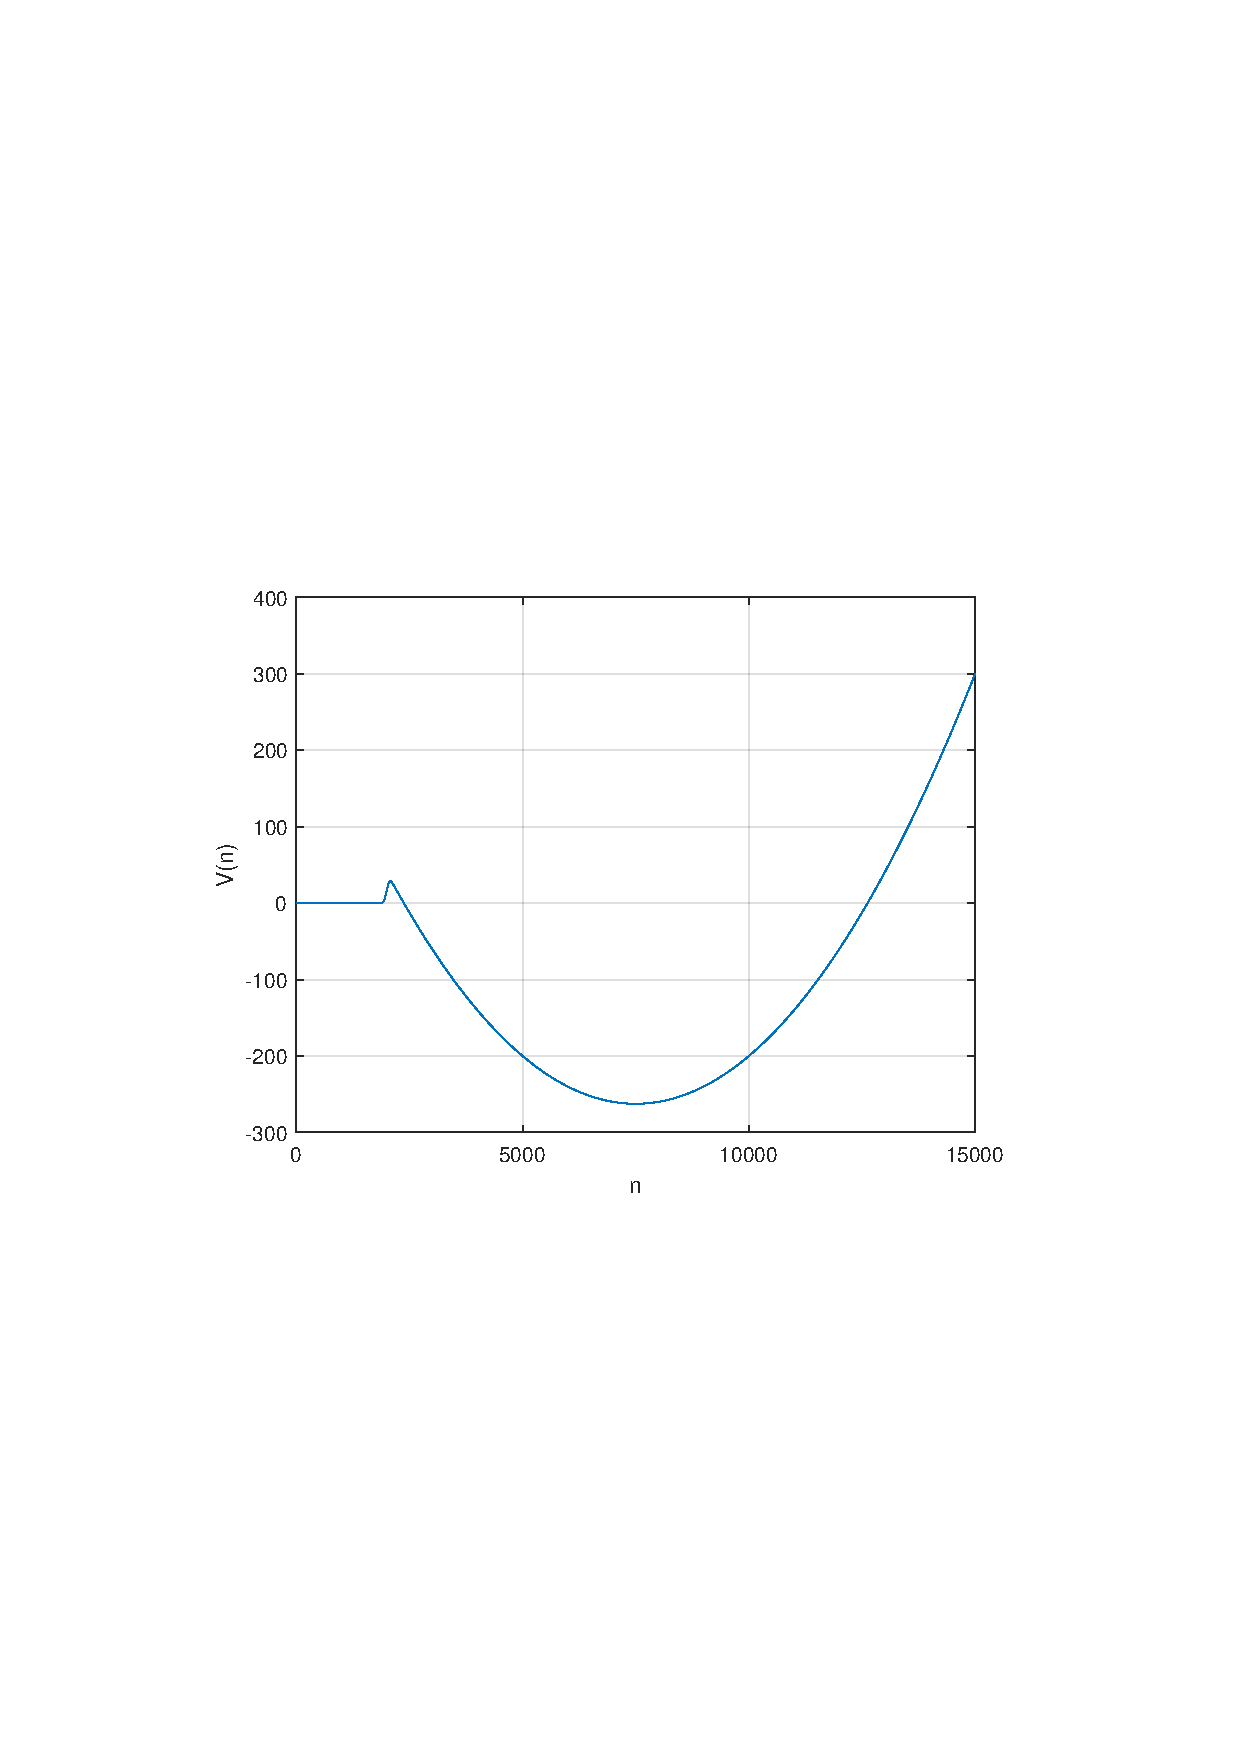
\includegraphics[width=0.8\textwidth,trim={3.09cm 9.295cm 3.09cm 9.295cm},clip]{fig/ex7_profit.pdf}
    \caption{利润$V$随购入报纸数量$n$变化的图像}
    \label{fig:ex7_profit}
\end{figure}

将$r$和$n$看作连续变量,则\Cref{eq:ex7_profit}可写作,
\begin{equation}
    V(n)=\int_0^n [(b-a) r-(a-c)(n-r)]f(r)dr + \int_n^{+\infty} (b-a)nf(r) dr
\end{equation}

注意这里$a$是关于$n$的函数,两边对$n$求导,化简得,
\begin{equation}
    V'(n) = \int_0^n \left(\frac{2An}{K}-A+c\right) f(r) dr + \int_n^{+\infty} \left(\frac{2An}{K}-A+b\right)f(r)dr
\end{equation}

令$V'(n)=0$,得到,
\begin{equation}
    \frac{\int_0^n f(r)dr}{\int_n^{+\infty} f(r)dr} = \frac{-2An+AK-bK}{2An-AK+cK}
\end{equation}

考虑到均值$\mu$比标准差$\sigma$大得多时,有$\int_0^n f(r)dr \approx \int_{-\infty}^n f(r)dr$,由对称性可知$\int_n^{+\infty} f(r)dr = 1-\int_{-\infty}^n f(r)dr$,因此得到,
\begin{equation}\label{eq:ex7_model}
    \int_{-\infty}^n f(r) dr = \frac{2An-AK+bK}{K(b-c)}
\end{equation}

\Cref{eq:ex7_model}即为本题的模型。

\paragraph{算法实现} \Cref{eq:ex7_model}是一个超越方程,无解析解,可采用\texttt{fzero}命令求解方程,采用\texttt{normcdf}命令计算正态分布的累积分布函数。

\subsubsection{程序}

请参见附录\ref{sec:ex7_code}。

\subsubsection{计算结果}

取初值为$n_0=2000$,计算得到最优购入报纸份数为$n=1968$。

\subsubsection{结果分析}

当限制$0 \le n \le 5000$时,批发价格$a$的取值范围为$0.45 \le a \le 0.5$,此时始终满足$c \le a \le b$,且批发价格与回收价格之间至少有0.1的差价,这是符合实际情况的。在这种限制下,求得的结果为全局最大值,可以作为实际应用的参考。

\subsubsection{结论}

为了获得最大利润,报童每天购进的报纸数应为1968份。


\section{收获与建议}

在本次实验中,我掌握了数据的参数估计方法,以及假设检验的基本原理和算法,用统计推断方法建立了实际问题的模型,并用MATLAB进行求解,在解决实际问题的过程中,我对数学方法的原理和应用有了更深刻的理解。

希望助教能对每次的实验进行详细的解答,希望老师在未来的课堂上介绍更多数学应用的前沿知识。

\section{附录:程序代码}

\subsection{Chap12-Ex5}\label{sec:ex5_code}

\lstinputlisting[language=Matlab]{../src/ex5.m}

\subsection{Chap12-Ex6}\label{sec:ex6_code}

\lstinputlisting[language=Matlab]{../src/ex6.m}

\subsection{Chap12-Ex7}\label{sec:ex7_code}

\lstinputlisting[language=Matlab]{../src/ex7.m}

\end{document}